\chapter{User Manual}

\section{Introduction}
The purpose of the system is to manage the restaurant in terms of orders and bookings more easily. The application enables the user to add, delete or update a booking and it enables the user to add or delete to an order and have the option to print or preview the invoice for the order. In addition, the user can manage the item menu by adding, deleting or updating an item from the menu.

\section{Installation}

\subsection{Software}
Since the application has been compiled into a windows executable (.exe), the user will not need to make any changes to their computer system or any additional software to run the application.

\subsection{Hardware}

The following hardware will be required to run the system:

\begin{itemize}

	\item A keyboard for user input
	\item A mouse to navigate around the application
	\item A Hard Disk Dirve for file storage 
	\item A Visual Display Unit for output
	\item A printer will be needed if the user wants to be able to print invoices
	

\end{itemize}



\subsection{Prerequisite Installation}

%include as many subsubsections as necessary for each piece of required software
\subsubsection{Installing Python}

\subsubsection{Installing PyQt}

\subsubsection{Etc.}

\subsection{System Installation}

The new system has been packaged into a windows installer and so to install the new system, follow these steps: \\
\\ 1. The install package is called "RestauranSetup", locate to the directory of the install package of where it has been placed. 

\begin{figure}[H]
    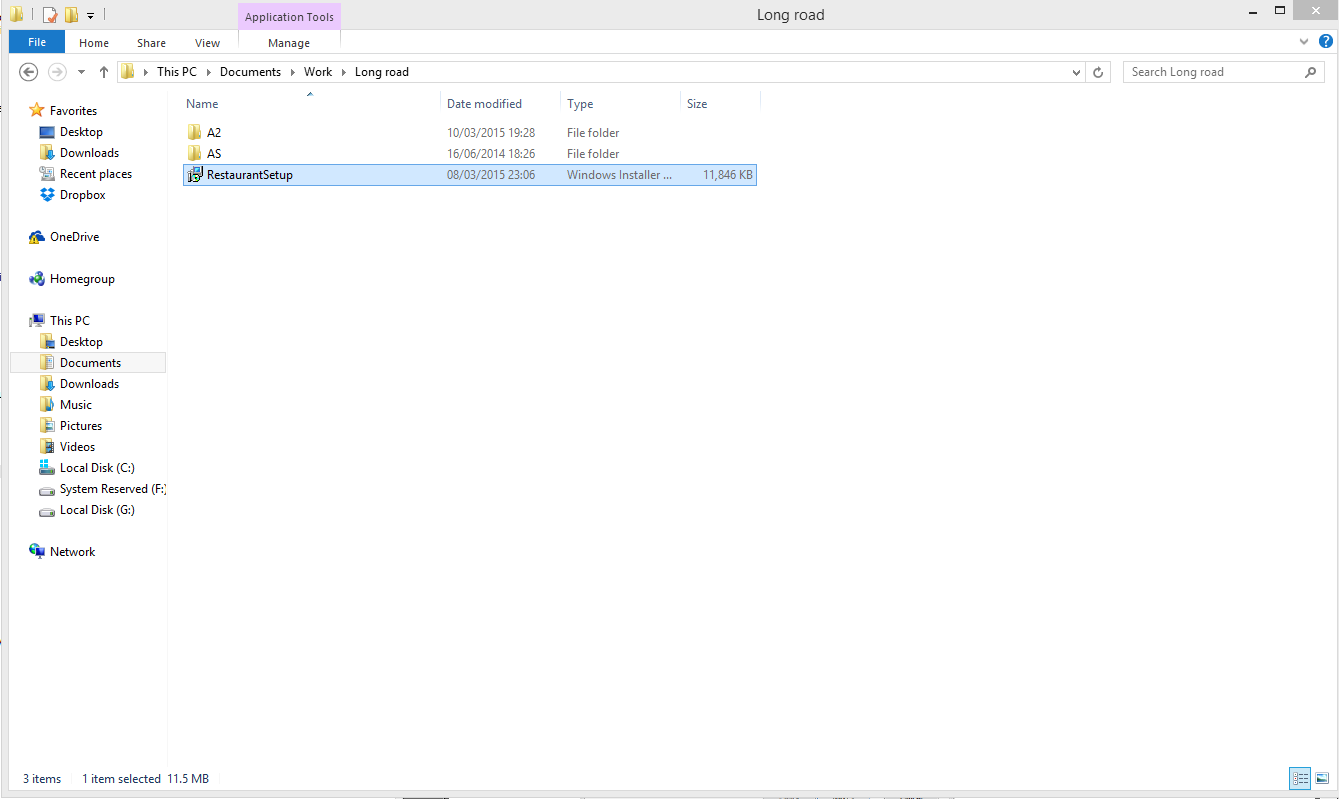
\includegraphics[height = 20cm]{./Manual/images/install1}
    \caption{Example of what the installer should look like} \label{fig:Flowchart1}
\end{figure}
\\

2. Double click on the installer and the 

\subsection{Running the System}

\section{Tutorial}

\subsection{Introduction}

\subsection{Assumptions}

\subsection{Tutorial Questions}

%include as many subsubsections as necessary for each question in your list
\subsubsection{Question 1}

\subsubsection{Question 2}

\subsection{Saving}

\subsection{Limitations}

\section{Error Recovery}

%include as many subsections as necessary for each error
\subsection{Error 1}

\subsection{Error 2}

\section{System Recovery}

\subsection{Backing-up Data}

\subsection{Restoring Data}